\begin{mainquestion}{energypowercharge}{Energy, Power, and Charge}

The energy absorbed by the BOX in the diagram is plotted in the graph below.

\begin{center}
    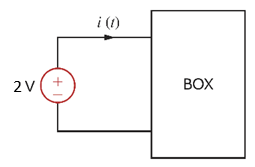
\includegraphics[width=0.5\textwidth]{schematic.png}
    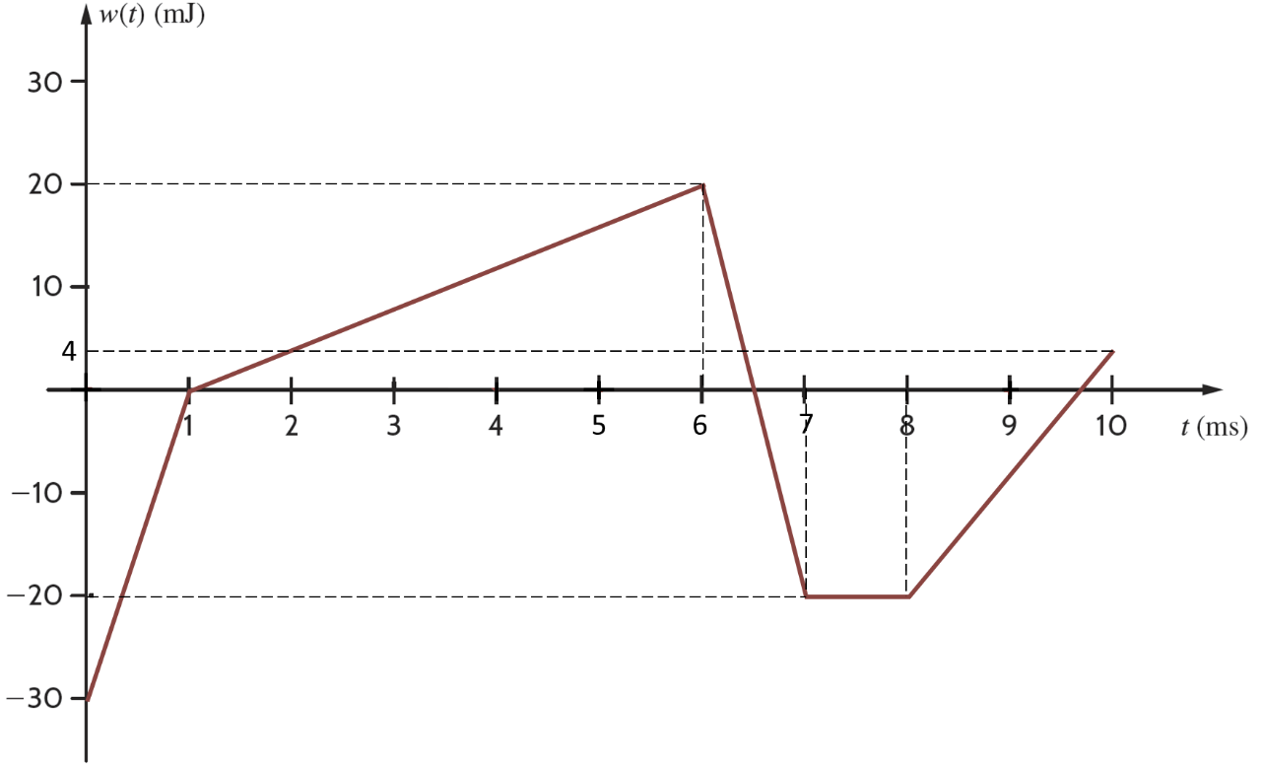
\includegraphics[]{waveform.png}
\end{center}

% =========================================================
\begin{partquestion}{current}
{Calculate and accurately sketch the current flowing into the box between 0 and \qty{10}{\milli\second}.}

\begin{answer}
Since $p(t)=\frac{\mathrm{d}w(t)}{\mathrm{d}t}$ , the power is just the slope of the energy absorbed by the BOX.  This can be readily determined from the provided graph, since the energy curve is piecewise linear.  We have:

\[
p(t)=
\left\{
\begin{matrix}
\frac{\qty{0}{\milli\joule}-\qty{-30}{\milli\joule}}{\qty{1}{\milli\second}-\qty{0}{\milli\second}}
= \qty{30}{\watt}
& 0<t<\qty{1}{\milli\second}
\\[6pt]
\frac{\qty{20}{\milli\joule}-\qty{0}{\milli\joule}}{\qty{6}{\milli\second}-\qty{1}{\milli\second}}
= \qty{4}{\watt}
& \qty{1}{\milli\second}<t<\qty{6}{\milli\second}
\\[6pt]
\frac{\qty{-20}{\milli\joule}-\qty{20}{\milli\joule}}{\qty{7}{\milli\second}-\qty{6}{\milli\second}}
= \qty{-40}{\watt}
& \qty{6}{\milli\second}<t<\qty{7}{\milli\second}
\\[6pt]
\qty{0}{\watt}
& \qty{7}{\milli\second}<t<\qty{8}{\milli\second}
\\[6pt]
\frac{\qty{4}{\milli\joule}-\qty{-20}{\milli\joule}}{\qty{10}{\milli\second}-\qty{8}{\milli\second}}
= \qty{12}{\watt}
& \qty{8}{\milli\second}<t<\qty{10}{\milli\second}
\end{matrix}
\right.
\]

This sketch is shown below:

\begin{center}    
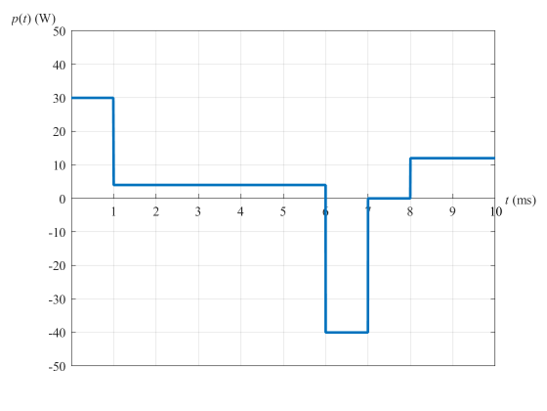
\includegraphics[width=0.8\textwidth]{power_sol.png}
\end{center}

\end{answer}
\end{partquestion}

% =========================================================
\begin{partquestion}{power}
{Calculate and accurately sketch the power flowing into the box between 0 and \qty{10}{\milli\second}.}

\begin{answer}
Since $p(t)=v(t)i(t)$ , the current flowing into the box is simply
$i(t)=\frac{p(t)}{v(t)}=\frac{p(t)}{\qty{2}{\volt}}$.
This can be written out as:

\[
i(t)=
\left\{
\begin{matrix}
\frac{\qty{30}{\watt}}{\qty{2}{\volt}}= \qty{15}{\ampere}
& 0<t<\qty{1}{\milli\second}
\\[6pt]
\frac{\qty{4}{\watt}}{\qty{2}{\volt}}= \qty{2}{\ampere}
& \qty{1}{\milli\second}<t<\qty{6}{\milli\second}
\\[6pt]
\frac{\qty{-40}{\watt}}{\qty{2}{\volt}}= \qty{-20}{\ampere}
& \qty{6}{\milli\second}<t<\qty{7}{\milli\second}
\\[6pt]
\frac{\qty{0}{\watt}}{\qty{2}{\volt}}= \qty{0}{\ampere}
& \qty{7}{\milli\second}<t<\qty{8}{\milli\second}
\\[6pt]
\frac{\qty{12}{\watt}}{\qty{2}{\volt}}= \qty{6}{\ampere}
& \qty{8}{\milli\second}<t<\qty{10}{\milli\second}
\end{matrix}
\right.
\]

The sketch is shown below:

\begin{center}    
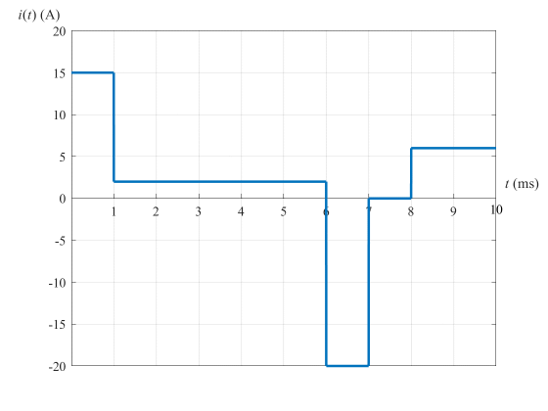
\includegraphics[width=0.8\textwidth]{current_sol.png}
\end{center}

\end{answer}
\end{partquestion}

% =========================================================
\begin{partquestion}{charge}
{What is the total charge delivered to the BOX during this same time interval?}

\begin{answer}
The total charge $Q$ delivered to the BOX is given by
$Q=\int_{0}^{\qty{10}{\milli\second}} i(t)\,\mathrm{d}t$.
This is simply the area under the current graph shown in part (b). The areas are calculated simply enough by summing together 4 rectangles (5 really, but one is of area 0!).  We have:
\begin{align*}
    Q &= (\qty{15}{\ampere})(\qty{1}{\milli\second})
    + (\qty{2}{\ampere})(\qty{5}{\milli\second})
    + (\qty{-20}{\ampere})(\qty{1}{\milli\second})
    + (\qty{0}{\ampere})(\qty{1}{\milli\second})
    + (\qty{6}{\ampere})(\qty{2}{\milli\second}) \\
    &= \qty{15}{\milli\coulomb}
    + \qty{10}{\milli\coulomb}
    - \qty{20}{\milli\coulomb}
    + \qty{0}{\milli\coulomb}
    + \qty{12}{\milli\coulomb} \\
    &= \qty{17}{\milli\coulomb}
\end{align*}
Incredible!

\end{answer}
\end{partquestion}

\end{mainquestion}